\section*{Two models of noise and skill}\label{2-models}

\subsection*{Notation}
Throughout this paper we use the following notation:
\begin{itemize}
    \item $i = 1,\ldots,N$ indexes cases (e.g., patient records, candidate waveforms)
    \item $j = 1,\ldots,M$ indexes raters
    \item $t = 1,\ldots,T$ indexes occasions (repeated ratings of the same case(s) by the same rater)
    \item $Y_{ijt}$ is the binary response (0 or 1) from rater $j$ on case $i$ at occasion $t$
\end{itemize}

We now explain the LTM and KSS models. Both models have this form: $Pr(Y_{ijt}=1) = f(z_{ijt})$, where $z_{ijt} = c_i + \ell_j + n_{ijt}$. Here, $Y_{ijt}=1$ represents a 'yes', 'positive', or 'correct' answer, depending on the context. The function $f$ can be either the logistic function $f(x) = 1/[1+\exp(-x)]$, or the cumulative Gaussian (probit) function $f(x) = (2\pi)^{-1/2}\int_{-\infty}^x \exp(-u^2/2)du$. The components of $z_{ijt}$ have somewhat different interpretations in the two models, which we explain below.

\subsection*{Latent Trait Model (LTM)}\label{section-LTM}
In the LTM,
\begin{eqnarray*}
  z_{ijt} &=& c_i + n_{ijt} \\
  Y_{ijt}&=&\begin{cases}
    1, & \text{if $z_{ijt}>\ell_j$}\\
    0, & \text{if $z_{ijt}\leq \ell_j$},
  \end{cases}
\end{eqnarray*}
where $c_i$ is the signal strength for case $i$ and $n_{ijt}$ is the noise. For an ideal observer, $z_{ijt} = c_i$, i.e., there is no noise ($n_{ijt}=0$). As indicated, decisions about the value of $Y_{ijt}$ are reached by comparing $z_{ijt}$ with a threshold value $\ell_j$ that is particular to rater $j$.

Note that a mathematically equivalent formulation is
\begin{eqnarray*}
  z_{ijt} &=& c_i - \ell_j + n_{ijt} \\
  Y_{ijt}&=&\begin{cases}
    1, & \text{if $z_{ijt}>0$}\\
    0, & \text{if $z_{ijt}\leq 0$},
  \end{cases}
\end{eqnarray*}
where we have absorbed $\ell_j$ into $z_{ijt}$. This form is consistent with the KSS model (see below) and with the logistic GLMM formulation where $\text{Pr}(Y_{ijt}=1) = f(c_i + \ell_j + n_{ijt})$.

In the LTM, $\ell_j$ represents the decision threshold of rater $j$: the minimum evidence level at which that rater classifies a case as positive. The noise $n_{ijt}$ represents uncertainty in the rater's perception or decision-making process. Historically, the LTM model has included the assumption that the noise depends only on the rater only, $n_{ijt} = n_j$, and has a Gaussian distribution with zero mean and standard deviation $\sigma_j$. We refer to the inverse of the noise standard deviation as the rater's 'skill' level, $s_j = 1/\sigma_j$, so that higher skill (smaller $\sigma_j$) means the rater is better able to discriminate between positive and negative cases (and hence has higher area under the ROC curve). 

In previous work, we have also referred to this model as the ``Similar Skill Individual Thresholds'' (SSIT) model, which makes the additional (testable) assumption that raters with similar levels of training tend to have a similar skill level but variable diagnostic thresholds, so that a single skill (or inverse noise) parameter describes responses for all raters in a group,  $\sigma_j = \sigma$. This application of the LTM model is illustrated below.

\subsubsection*{Empirical validation: Expert detection of interictal epileptiform discharges}

To illustrate the LTM framework, we applied it to a study of routine and scalp EEG waveform interpretation. Twenty-nine neurophysiology specialists with varying levels of expertise (9 board-certified epilepsy experts, 7 experienced non-experts, and 13 novices) independently classified a large number (>1000) of candidate waveforms extracted from continuous scalp EEG recordings as either interictal epileptiform discharges (IEDs, also called "spikes") or non-IED waveforms.

Figure~\ref{fig:ltm-model} illustrates the decision-making process assumed by the model (Panel A) and the resulting classification patterns across the range of evidence strength (Panel B). The model was fit to estimate each individual's skill level (inverse noise: $s_j = 1/\sigma_j$) and decision threshold ($\ell_j$). Results shown in Figure~\ref{fig:ltm-roc} A demonstrate systematic differences in noise levels across expertise groups: experts exhibited lower noise (median $\sigma = 1.262$, corresponding to higher skill) compared to novices (median $\sigma = 2.664$). This difference in skill translates to superior discrimination performance, with experts achieving a median AUC of 0.891 compared to novices' median AUC of 0.735. 

\begin{figure}[htbp]
\centering
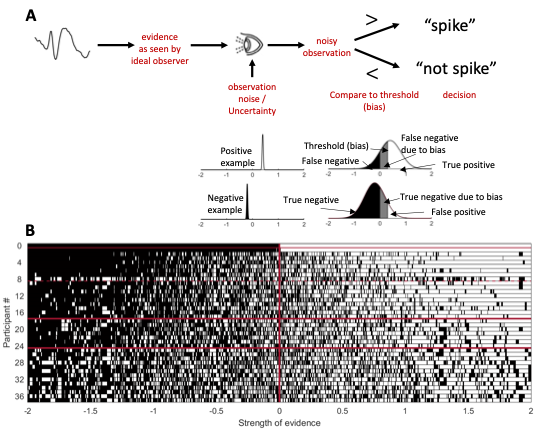
\includegraphics[width=0.75\textwidth]{Fig1-Noise-Model.png}
\caption{The LTM decision model applied to expert detection of interictal epileptiform discharges in EEG recordings. \textbf{Panel A:} Schematic of the signal detection process assumed in the LTM model. For each candidate waveform, an ideal observer would perceive the true evidence level ($c_i$). Each rater in effect receives a noisy observation ($z_{ijt} = c_i + n_{ijt}$) contaminated by perceptual or decision noise with standard deviation $\sigma_j$. The rater compares this noisy observation to their personal threshold ($\ell_j$) to produce a binary classification (IED vs. non-IED). Lower noise (higher skill $s_j = 1/\sigma_j$) produces observations closer to the true signal. \textbf{Panel B:} Heatmap showing classification decisions across 37 raters (rows) and the full range of evidence strength (columns, from strong evidence against IED on left to strong evidence for IED on right). White indicates "IED" classification; black indicates "non-IED" classification. Raters are sorted by estimated skill level (top = highest skill/lowest noise). High-skill raters show sharper transitions from black to white at consistent evidence levels, while lower-skill raters show more gradual, variable transition zones, reflecting greater noise in their decision-making.}
\label{fig:ltm-model}
\end{figure}

\begin{figure}[htbp]
\centering
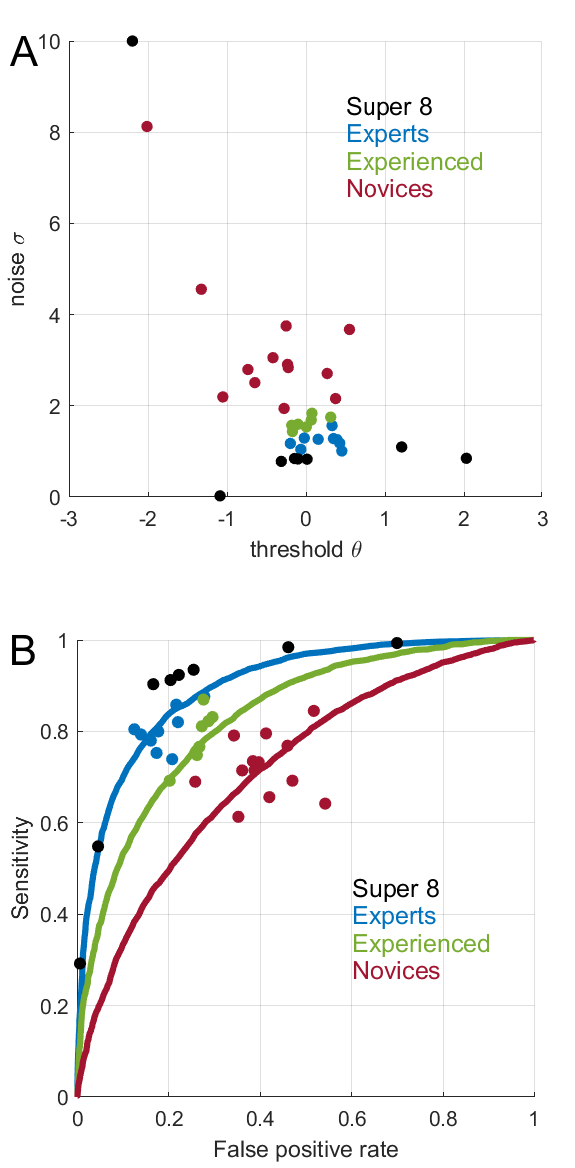
\includegraphics[width=0.5\textwidth]{SSIT-ROCs.png}
\caption{Estimated LTM parameters and resulting ROC curves by expertise level. \textbf{Panel A:} Distribution of estimated internal noise levels ($\sigma$, y-axis) and decision thresholds ($\theta$, x-axis) for each rater. Black points ('Super 8') represent 8 experts who participated in an early IED annotation study; blue points ('Experts') show additional board-certified experts who participated in a later annotation study; green points show experienced non-experts; red points show novices. Experts cluster in the low-noise region ($\sigma \approx 1$--$2$), while novices are distributed across higher noise levels ($\sigma \approx 2$--$10$). Threshold values vary across the full range for all groups, indicating that expertise affects discrimination ability (noise level) more than diagnostic bias (threshold). \textbf{Panel B:} Group-level ROC curves reconstructed from estimated parameters. Each point represents an individual rater's operating point (sensitivity vs. false positive rate). The smooth curves show the group-average ROC curves: experts (blue) achieve superior discrimination (AUC $\approx$ 0.89), experienced non-experts (green) show intermediate performance (AUC $\approx$ 0.85), and novices (red) exhibit substantially lower discrimination ability (AUC $\approx$ 0.74).}
\label{fig:ltm-roc}
\end{figure}

Grouping raters by expertise levels (Figure~\ref{fig:ltm-roc}), we see that their operating points cluster near the group-median ROC curves, suggesting that raters with similar training levels indeed have similar skill levels (Panel B). Nevertheless, decision thresholds ($\ell_j$) vary widely even among experts (Panel A), indicating that while discrimination ability is governed by level of expertise, variation in decision thresholds is a major source of between-expert disagreement for this diagnostic task. These findings show that the LTM framework successfully separates two distinct dimensions of rater performance: skill (captured by noise level $\sigma_j$, which determines the ROC curve and its AUC) and bias (captured by threshold $\ell_j$, which determines the operating point on that curve).

\subsubsection*{ROC curves, skill, and noise in the LTM}\label{section-ROC}
When working with the LTM, we assume that the correct answer $C$ for each case is available, either via an external gold standard or by taking the correct answer to be the group consensus. Each rater response can then be categorized as true positive, true negative, false positive, or false negative. We specify the percentage of positive cases ($C=1$) that the rater correctly labeled as such, known as the sensitivity $Se = Pr(Y_{ijt}=1|C=1)$, and the percentage of negative cases ($C=0$) that the rater incorrectly labeled as positive, known as the false positive rate $Fp = Pr(Y_{ijt}=1|C=0)$.

Recall that in the LTM the rater's answers $Y_{ijt}$ are determined by comparing $z_{ijt} = c_i + n_{ijt}$ with a threshold $\ell_j$. Denote the mean values of $z_{ijt}$ when $C=0$ as $\mu_0$, and the mean when $C=1$ as $\mu_1$. Assume the standard deviation of $z_{ijt}$ is $\sigma$f for both $C=1$ and for $C=1$. Then we can write the sensitivity and false positive rates as functions of $\ell_j$, $\mu_0$, $\mu_1$:
\begin{eqnarray*}
    Se(\ell_j) &=& Pr(c_{i}+n_{ijt}>\ell_j|c_{i}>0) = \Phi\left(\frac{\mu_1-\ell_j}{\sigma}\right)\\
    Fp(\ell_j) &=& Pr(c_{i}+n_{ijt}>\ell_j|c_i \leq 0) = \Phi\left(\frac{\mu_0-\ell_j}{\sigma}\right).
\end{eqnarray*}
where $\Phi$ is the standard normal cumulative distribution function. The ROC curve is the set of points $(Se, Fp)$ formed by allowing the threshold $\ell_j$ to range over all possible values. We see that each rater has a unique operating point $(Se(\ell_j), Fp(\ell_j))$ determined by their threshold. The area under the ROC curve (AUROC) is given by

$$AUROC = \Phi\left(\frac{\mu_1-\mu_0}{\sigma \sqrt{2}}\right).$$

This formulation reveals the connection between noise and discrimination: smaller $\sigma$ (higher skill) leads to higher AUROC, while the threshold $\ell_j$ determines the operating point on the ROC curve without affecting the AUROC.

\subsection*{KSS Noise decomposition}\label{section-KSS}
In the Kahneman-Sibony-Sunstein (KSS) noise decomposition framework, $$z_{ijt} = c_i + \ell_j + p_{ij} + o_{ijt},$$
where $c_i$ represents variation due to differences in case information (signal), and the other terms represent noise: $\ell_j$ is level noise, the tendency of rater $j$ to answer 'yes' or classify cases as "1" regardless of case-specific evidence; $p_{ij}$ is pattern noise, reflecting the idiosyncratic way that rater $j$ views the information in case $i$; and $o_{ijt}$ is occasion noise, reflecting differences in the response of rater $j$ to case $i$ on different occasions $t$.

Note that the total noise term $n_{ijt}$ from the LTM has been decomposed into two parts: $n_{ijt} = p_{ij} + o_{ijt}$. Each of the terms $c_i$, $\ell_j$, $p_{ij}$, $o_{ijt}$ is modeled as an independent Gaussian random variable with zero mean and standard deviations $\sigma_c$, $\sigma_\ell$, $\sigma_p$, $\sigma_o$, respectively. 

\begin{figure}[h!]
\begin{center}
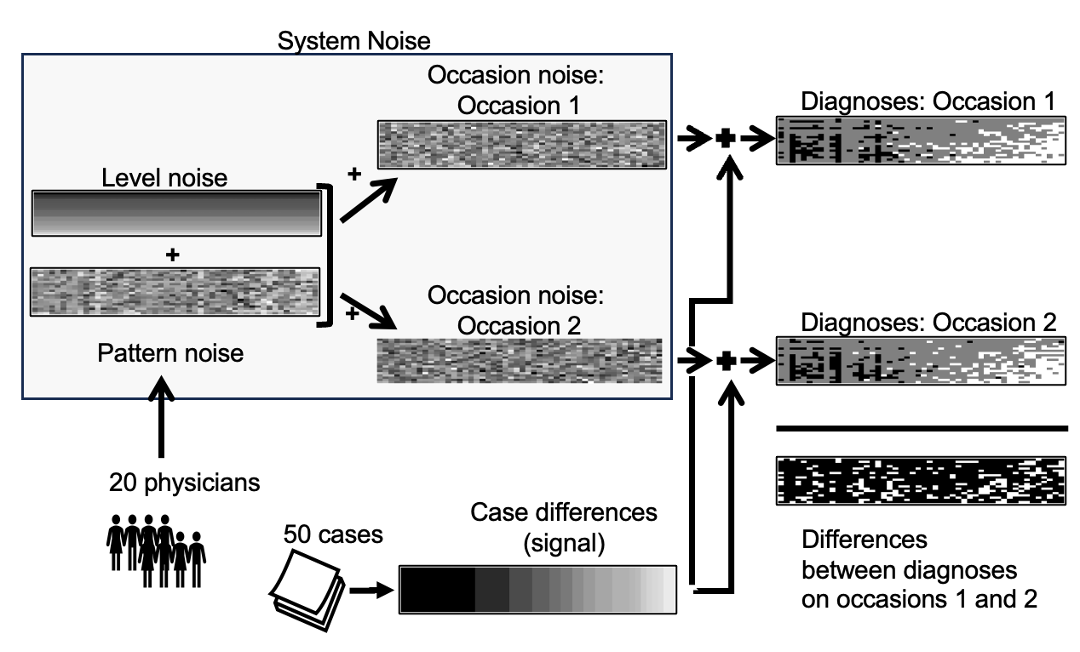
\includegraphics[width=0.70\columnwidth]{KSS-Model.png}
\caption{{\textbf{Noise decomposition: KSS framework} Illustration of how the KSS model accounts for variation in expert response data about cases histories in patients with suspected epilepsy.The three panels on the right show actual data, while the 5 on the left are estimated from the data using the KSS framework. Variation in expert responses is decomposed into signal (information intrinsic to the cases), and system noise. System noise is further decomposed into level noise, pattern noise, and occasion noise. These different types of noise are combined additively with the signal to reach a final decision. The heatmaps show the actual estimates. 
{\label{Fig3-KSS}}%
}}
\end{center}
\end{figure}

The ROC curve formulation described in the LTM section can be extended to the KSS model by treating the sum of pattern and occasion noise as total noise: $n_{ijt} = p_{ij} + o_{ijt}$, with variance $\sigma^2 = \sigma_p^2 + \sigma_o^2$. This allows computation of AUROC and rater operating points in the full KSS framework, where discrimination depends on the total noise magnitude rather than its decomposition into pattern and occasion components.

\subsection*{Unified Framework: Relating LTM and KSS}\label{section-unified}

The two models described above---LTM and KSS---are special cases of a single unified framework. Both can be expressed as generalized linear mixed models (GLMMs) with a logistic (or probit) link function:

\begin{equation}
\label{eq:master-model}
\boxed{
\begin{aligned}
Y_{ijt} &\sim \text{Bernoulli}(\pi_{ijt}) \\
\text{logit}(\pi_{ijt}) &= c_i + \ell_j + p_{ij} + o_{ijt} + \bar{y}
\end{aligned}
}
\end{equation}

where all random effects are independent and normally distributed:
$$c_i \sim \mathcal{N}(0,\sigma_c^2), \quad \ell_j \sim \mathcal{N}(0,\sigma_\ell^2), \quad p_{ij} \sim \mathcal{N}(0,\sigma_p^2), \quad o_{ijt} \sim \mathcal{N}(0,\sigma_o^2).$$

\textbf{Clinical interpretation of model components:}
\begin{itemize}
    \item $c_i$ = \textbf{Evidence in the case} (e.g., clarity of patient history, strength of EEG findings)
    \item $\ell_j$ = \textbf{Expert's personal diagnostic threshold} (tendency to over- or under-diagnose relative to peers)
    \item $p_{ij}$ = \textbf{Expert's idiosyncratic interpretation} of specific case features (stable across time)
    \item $o_{ijt}$ = \textbf{Expert inconsistency across occasions} (mood, fatigue, time of day)
    \item $\bar{y}$ = \textbf{Overall base rate} (population prevalence on logit scale)
\end{itemize}

The two models differ in how they treat discrimination noise:

\begin{itemize}
    \item \textbf{LTM:} Pattern and occasion noise are not separated; instead, $n_{ijt} = p_{ij} + o_{ijt}$ is treated as a single combined noise term with variance $\sigma^2 = \sigma_p^2 + \sigma_o^2$. This model includes case signal ($c_i$), rater thresholds ($\ell_j$), and total discrimination noise, but does not explicitly decompose noise into pattern and occasion components. The LTM is typically applied when repeated measurements (multiple occasions) are not available or when the decomposition of discrimination noise into pattern vs. occasion components is not of primary interest.

    \item \textbf{KSS (full model):} This model decomposes variation into signal ($c_i$), level noise ($\ell_j$), pattern noise ($p_{ij}$), and occasion noise ($o_{ijt}$). KSS requires repeated measurements to separate pattern noise (stable across occasions for a given rater-case pair) from occasion noise (varies across occasions).
\end{itemize}

This unified view clarifies that:
\begin{enumerate}
    \item Both models share the same underlying structure (Equation~\ref{eq:master-model})
    \item They differ only in model complexity, with KSS being more general
    \item Model selection depends on the data structure (e.g., whether repeated measurements are available) and research questions (e.g., whether separating pattern from occasion noise is important)
    \item Both models can be estimated using the same statistical framework (hierarchical Bayes or mixed-effects maximum likelihood)
\end{enumerate}

\section*{Interpretation of model parameters on the group and individual levels}\label{section-interpretation}
The KSS model is the most general of the two models, containing the LTM as a special case. Here we summarize the quantities needed to provide a full description of a set of response data within the KSS model, and their interpretation. The interpretations involve two levels: the individual and the group level.

\begin{itemize}
    \item \textbf{Individual level interpretation:}
    \begin{itemize}
    \item $c_i$ quantifies the signal, or strength of the evidence in case $i$. Larger values imply stronger evidence that the correct answer or label for case $i$ is 1, and more negative values imply stronger evidence that the correct answer is 0.
    \item $\ell_j$ quantifies the 'bias' or 'threshold' of rater $j$---the tendency to either over-call or under-call. This parameter determines the rater's operating point on a receiver-operating characteristic curve. Unlike the other parameters, $\ell_j$ represents a consistent tendency of rater $j$ that is independent of the information in any particular case $i$. From the perspective of an individual rater, this tendency is not 'noise' because it is consistent and stable across cases and occasions. However, from the perspective of the group, $\ell_j$ varies across raters and is unrelated to case-specific information; thus at the group level $\ell_j$ is noise.
    \item $p_{ij}$ quantifies pattern noise: the idiosyncratic way rater $j$ weights the information in case $i$ as favoring (when positive) or being against (when negative) labeling case $i$ as 1. For rater $j$, this response is stable across occasions: each time the rater sees case $i$, the model predicts the answer will be skewed in the same way. From the perspective of the individual rater, this tendency is not 'noise' because it is consistent across occasions. However, from the perspective of the group, $p_{ij}$ varies across raters; thus at the group level $p_{ij}$ is noise.
    \item $o_{ijt}$ quantifies the occasion noise, or variation in the response of rater $j$ to case $i$ on different occasions $t$. This quantity is considered noise at both the individual and group levels, because $o_{ijt}$ varies not only across raters but also within raters (the same rater labels the same case differently on different occasions).
    \end{itemize}
    \item \textbf{Group level interepretation:}
    \begin{itemize}
        \item $c_i$ varies across cases $i$, leading to variation in responses that is related to the underlying case information or 'signal'. This variation is modeled as $c_i \sim \mathcal{N}(0,\sigma_c^2)$.
        \item $\ell_j$ represents noise at the group level because it varies across raters $j$, independent of the underlying information $c_i$, leading the 'system' of raters to provide variable responses to the same case. This variation is modeled as $\ell_j \sim \mathcal{N}(0,\sigma_\ell^2)$.
        \item $p_{ij}$ represents noise at the group level because it varies across cases $i$ and raters $j$, independent of the underlying information $c_i$. This variation is modeled as $p_{ij} \sim \mathcal{N}(0,\sigma_p^2)$.
        \item $o_{ijt}$ represents noise at both the individual and group levels, as explained above. This variation is modeled as $o_{ijt} \sim \mathcal{N}(0,\sigma_o^2)$.
    \end{itemize}
\end{itemize}

If the number of cases is $N$, the number of raters is $M$, and the number of occasions is $T$, then the total number of responses $Y_{ijt}$ collected is $N \cdot M \cdot T$. The quantities required to fully describe the data are the actual values of the underlying variables $c_i$, $\ell_j$, $p_{ij}$, $o_{ijt}$, and the standard deviations $\sigma_c$, $\sigma_\ell$, $\sigma_p$, $\sigma_o$. Thus the total number of variables to be estimated is $N + M + N \cdot M + N \cdot M \cdot T + 4$.

All of these quantities may be of interest, or only a subset, depending on the research goals. In some cases, we may be interested only in estimating the noise magnitudes and comparing them with the signal strength; the quantities to be estimated are then $\sigma_c$, $\sigma_\ell$, $\sigma_p$, $\sigma_o$. In other cases, the aim may be to characterize the skill and decision thresholds of a group of raters with similar skill levels; the quantities of interest may be $c_i$, $\ell_j$, and the variance of the noise $\sigma$. This case is the subject of the LTM.

\section*{Identifiability and Scale}\label{section-identifiability}

Understanding the scale and identifiability of the model parameters is important for correct interpretation. This section addresses common sources of confusion.

\subsection*{The latent scale is not fully identified}

In our model, only binary outcomes $Y_{ijt} \in \{0,1\}$ are observed. The underlying latent variable $z_{ijt} = c_i + \ell_j + p_{ij} + o_{ijt} + \bar{y}$ is continuous and unobserved. Because we observe only the binary outcomes via the link function $\text{Pr}(Y_{ijt}=1) = f(z_{ijt})$, the absolute scale of the latent variable is not identified.

In the logistic model with link function $f(x) = 1/(1+\exp(-x))$, the residual variance is implicitly fixed by the link function. Specifically, the logistic distribution has variance $\pi^2/3 \approx 3.29$, which acts as an implicit scale constraint. All variance components $\sigma_c^2, \sigma_\ell^2, \sigma_p^2, \sigma_o^2$ are expressed relative to this latent scale.

In the probit model with link function $f(x) = \Phi(x)$ (standard normal CDF), the residual variance is implicitly 1. Results from logistic and probit models differ by a rescaling factor of approximately $\sqrt{\pi^2/3} \approx 1.81$.

\subsection*{Practical consequences}

\begin{enumerate}
    \item \textbf{Variance decomposition is on the latent scale.} When we report that signal accounts for X\% of total variation, this percentage is computed on the logit (or probit) scale, not on the probability scale. The latent-scale decomposition is:
    $$\text{Total Variance} = \sigma_c^2 + \sigma_\ell^2 + \sigma_p^2 + \sigma_o^2$$
    $$\text{\% Signal} = \frac{\sigma_c^2}{\sigma_c^2 + \sigma_\ell^2 + \sigma_p^2 + \sigma_o^2} \times 100$$

    \item \textbf{Variance decomposition on the probability scale requires simulation.} If you want to know "what percentage of variation in predicted probabilities is due to signal vs. noise," you must use posterior predictive simulation to compute predictions on the probability scale and then decompose their variance. This is more complex and depends on the distribution of cases (e.g., prevalence).

    \item \textbf{Absolute magnitudes of $\sigma$ values depend on the link function.} A value of $\sigma_c = 2$ in a logistic model corresponds roughly to $\sigma_c \approx 1.1$ in a probit model. However, the \textit{relative} contributions (percentages) are invariant to this rescaling.

    \item \textbf{Comparisons across studies require the same link function.} When comparing noise levels across studies, ensure both use logistic (or both use probit) links. Alternatively, report standardized effect sizes or percent contributions.

    \item \textbf{Alternative anchoring strategies.} Some researchers fix $\text{Var}(c_i) = 1$ or $\text{Var}(\ell_j) = 1$ to anchor the scale. This is a valid alternative; results differ only by rescaling. We do not adopt this approach because the logistic link provides a natural implicit anchor.
\end{enumerate}

\fbox{\begin{minipage}{0.95\textwidth}
\textbf{Key Point:} All variance components are on the latent (logit or probit) scale, not the probability scale. Percent variance contributions are interpretable and comparable within a study. For cross-study comparisons or probability-scale interpretations, use posterior predictive simulation.

\textbf{Connection to the epilepsy case study:} While we report variance components on the latent logit scale (e.g., level noise = 23\% of latent variance in Stage 1), the practical impact is seen in observable outcomes: the 16\% occasion reversal rate and 26\% inter-expert disagreement rate. The latent-scale decomposition allows us to understand \textit{why} these observable disagreements occur, but the framework's value lies in connecting abstract variance components to concrete clinical phenomena.
\end{minipage}}

\subsection*{When can one reliably estimate pattern noise?}

The pattern noise term $p_{ij}$ is a rater-by-case interaction. Estimating $\sigma_p$ requires sufficient data structure:

\begin{itemize}
    \item \textbf{Many raters AND many cases:} Pattern noise reflects how rater $j$'s response to case $i$ deviates from the additive effects of $c_i$ and $\ell_j$. To separate this interaction from residual noise, you need substantial cross-classification (many raters $\times$ many cases).

    \item \textbf{Replication helps:} If $T \geq 2$ (repeated occasions), the model can better separate pattern noise $p_{ij}$ (stable across occasions for a given rater-case pair) from occasion noise $o_{ijt}$ (varies across occasions).

    \item \textbf{With $T=1$ (single rating per rater-case pair):} The model can still estimate $\sigma_p$ via hierarchical shrinkage, but the estimate is weakly identified and relies heavily on the prior. Pattern and occasion noise in this situation are partially confounded.

\end{itemize}
